\documentclass[12pt]{article}
\usepackage{amsmath}
\usepackage{amsfonts}
\usepackage{mathrsfs}
\usepackage{lscape}
\usepackage{listings}
\usepackage{graphicx} % Allows for importing of figures
\usepackage{color} % Allows for fonts to be colored
\usepackage{comment} % Allows for comments to be made
\usepackage{accents} % Allows for accents to be made above and below text
%\usepackage{undertilde} % Allows for under tildes to take place for vectors and tensors
\usepackage[table]{xcolor}
\usepackage{array,ragged2e}
\usepackage{hyperref}
\usepackage{framed} % Allows boxes to encase equations and such
\usepackage{subcaption} % Allows for figures to be side-by-side
\usepackage{float} % Allows for images to not float in the document
\usepackage{booktabs}
%\usepackage[margin=0.75in]{geometry}
\usepackage[final]{pdfpages}
\usepackage{enumitem}
\usepackage[section]{placeins}

%%%%%%%%%%%%%%%%%%%%%%%%%  Function used to generate vectors and tensors %%%%%%%%%
\usepackage{stackengine}
\stackMath
\newcommand\tensor[2][1]{%
	\def\useanchorwidth{T}%
	\ifnum#1>1%
	\stackunder[0pt]{\tensor[\numexpr#1-1\relax]{#2}}{\scriptscriptstyle \sim}%
	\else%
	\stackunder[1pt]{#2}{\scriptscriptstyle \sim}%
	\fi%
}
%%%%%%%%%%%%%%%%%%%

\definecolor{mygrey}{rgb}{0.97,0.98,0.99}
\definecolor{codeblue}{rgb}{.2,0,1}
\definecolor{codered}{rgb}{1,0,0}
\definecolor{codegreen}{rgb}{0.3,0.33,0.12}
\definecolor{codegray}{rgb}{0.5,0.5,0.5}
\definecolor{codepurple}{rgb}{0.55,0.0,0.55}
\definecolor{codecyan}{rgb}{0.0,.4,.4}

\lstdefinestyle{mystyle}{
	backgroundcolor=\color{mygrey},   
	commentstyle=\color{codegreen},
	keywordstyle=\color{codeblue},
	stringstyle=\color{codepurple},
	numberstyle=\tiny\color{codegray},
	basicstyle=\footnotesize,
	breakatwhitespace=false,         
	breaklines=true,                 
	captionpos=b,                    
	keepspaces=true, 
	numbers=left,                    
	numbersep=5pt,                  
	showspaces=false,                
	showstringspaces=false,
	showtabs=false,                  
	tabsize=2
}
\lstset{style=mystyle}

\lstset{language=Matlab,backgroundcolor=\color{mygrey}}
\usepackage{lastpage}
\usepackage{fancyhdr}
\pagestyle{fancy}
%\lhead{\large{Nik Benko, John Callaway, Nick Dorsett, Martin Raming}} 
%\chead{\large{\textbf{ME EN 6960: Lab 1}}}
%\rhead{\today}
\cfoot{[\thepage\ of \pageref{LastPage}]}
\fancyheadoffset{.5cm}
\setlength{\parindent}{0cm}
\usepackage[left=.5in, right=0.50in, top=1.00in,bottom=1.00in]{geometry}
\usepackage{microtype} 
\usepackage{setspace}
\doublespace
%%%%%%%%%%%%%%%%%%%%%%%%%%%%%%%%%%%%%%%%%%%%%%%%%%%%%%%%%%%%%%%%%%%%%%%%%%


\begin{document}
\title{ Analysis of Stress Intensity Factors for Mode I and Mixed Mode with Digital Image Correlation \\ \normalsize{ME EN 6960}}
\author{Nik Benko, John Callaway, Nick Dorsett, Martin Raming}
\maketitle


\begin{abstract} 
	Failure in a material is often dependent on the presence of flaws within the part. In this experiment, Digital Image Correlation was used to analyze the displacement of a thin sheet of PMMA with an induced edge crack within a symmetric three point bend configuration. This test was then repeated using an asymmetric three point bend configuration to produce a set of data under mixed mode loading. The Westergaard stress function solution for an edge crack was used to compute the stress intensity factors for each data set, and the Mode 1 data was compared to an analytical solution calculated with strength of materials equations. 
\end{abstract}

\section{Introduction} %Nick

When a material fails, the theoretical stress required to break the molecular bonds is less than the ultimate stress. This occurs because of geometric features, such as cracks, which cause stress concentrations that magnify the effect of applied loads. Classical strengths of materials equations are useful for producing general solutions to problems, but in order to analyze specific cases in detail, Linear Elastic Fracture Mechanics (LEFM) are used instead. LEFM assumes that cracks are inherently present in a material, that a crack is a free surface within the surrounding stress field, the elastic solution surrounding this crack is based on a stress intensity factor K, and that the stress on the crack tip can be used to predict the crack propagation. Furthermore, the area surrounding a crack consists of three major parts. The first part, consisting of the crack tip, is a region of plastic deformation at which it is not valid to use LEFM due to the plastic deformation there. The second region is the linear elastic region, where LEFM is applied in describing the stress state of the material. The third section is the far field where the stress state is no longer affected by the presence of the crack. By analyzing the second region, information on the stress intensity factor can be determined for a variety of loads.
\\
\\
In previous works, such as that of Dally and Sanford (citation), strain gauges were used to capture displacement around crack tips. While strain gauges are useful in providing displacement data, they also only are valid over the region directly underneath the gauge, limiting the information provided. Optical techniques, however, can be used to provide the full-field displacement data surrounding a crack. This data is useful because through analyzing the contours present in full-field data, it can be determined what mode in which the crack is loaded as well as provides a more complete data set for analysis. Photoelasticity and Moire Inferometry have been used successfully to measure the to capture material behavior. Digital image correlation is attractive method because it is applicable on most materials, does not require any particularly complicated equipment, and is easy to set up and use.
\\
\\
This paper describes the use of digital image correlation (DIC) to capture displacement data around a crack tip when it undergoes pure Mode 1 loading and mixed Mode 1 and Mode 2 loadings. Using this information, the stress intensity factors are calculated using the Westergaard stress function solution for both Mode 1 and mixed mode loads. (Dally and Sanford). These calculated stress intensity factors from LEFM are then compared to the analytical solution for the given loading scenario.

\section{Methods}

\subsection{Experimental Techniques} 

\subsubsection{Digital Image Correlation} % Martin
DIC is a commonly used optical technique in experimental mechanics to accurately measure full-field displacements, and rotations by capturing a sequence of images of a the surface in question. Using two cameras these measurements can be taken in 3D. If only 2D measurements are needed, as in this experiment, only one camera is needed for imaging the surface.
\\
\\
An initial digital image is taken to be used as the reference image which is done before any significant loading of the specimen occurs. Here it is assumed that displacements, and rotations are nearly zero.  This reference image is then compared to a digital image taken once loading has occurred, also know as the deformed image. In many cases numerous digital images are captured during loading for comparison to create a sequence of displacements and rotations.  For correlation to take place an area of interest with in the images is selected and then divided into square sections known as subsets. Each subset is made up of the same number of pixels.  The subsets are matched from the deformed images to the reference image though a correlation function with in the DIC algorithm. By corresponding each pixel to an actual unit of length deformations and rotations can then be tracked using a DIC algorithm \cite{DIC}.
\\
\\
For the DIC algorithm to be effective each subset must contain enough unique features.  These features are related to contrast or pixel values with in each subset. A high-contrast uniform granular  surface is desired to create such usable features. In practice this is known as a speckle pattern. A usable speckle pattern consists of uniformly dispersed speckles of  random shapes and varying sizes. The size of the speckles needed will depend on the size of the specimen and focusing distances. For example, a small specimen with the camera close will require very small speckles while a larger specimen with the camera backed off requires larger speckles. 

\subsubsection{Experimental Determination of Displacement Fields} %John
Mode 1 displacement fields can be obtained by loading a specimen that has an edge crack in a three point configuration. This configuration and specimen geometry is given in Figure \ref{fig:Geometry}. Alignment of the roller directly above the crack tip creates pure bending around the crack, which induces only mode I crack opening, and therefore mode I displacement fields.
\\ \\
Mixed mode displacement fields can be obtained by inducing eccentricity in the previously described three point loading configuration. This can be done by moving one of the lower support rollers, creating a combination of bending (Mode I) and shear (Mode II) around the crack. This configuration is given in Figure \ref{fig:Geometry_Mixed}.  

\subsubsection{Calculation of Stress Intensity Factors} %john - still need to add references
Theoretical mode I stress intensity factors ($K_{I}$) can be calculated using the closed form equation:
\begin{equation}
K_{I} = Y\sigma\sqrt{\pi a}
\end{equation}
where $\sigma$ is the farfield stress, a is the crack length and Y is a geometric factor specific to the loading configuration and specimen geometry. Using the solution developed in \textit{The Stress Analysis of Cracks Handbook}, the stress intensity factor for the single edge notched bend specimen being examined is:
\begin{equation}
K_{I} = \frac{P}{B\sqrt{W}}\Bigg(\frac{\frac{3S}{W}\sqrt{\frac{a}{w}}}{2(1+\frac{2a}{w})(1-\frac{a}{w})^{1.5}}\Bigg)\Bigg[1.99-\frac{a}{w}\Big(1-\frac{a}{w}\Big)\Big[2.15-3.93\Big(\frac{a}{w}\Big)+2.7\Big(\frac{a}{w}\Big)^2\Big]\Bigg]
\end{equation}
where P is the applied load, W is the specimen width, B is the specimen thickness and a is the crack length. 
\\ \\
Experimental mode I stress intensity factors can be found using the experimental displacement fields. From the Westergaard solution, the displacements around the crack can be described by the following equations:
\begin{equation}
u_{x} = \frac{K_{I}}{8\mu \pi}\sqrt{2\pi r}\bigg[(2\kappa-1)cos\bigg(\frac{\theta}{2}\bigg)-cos\bigg(\frac{3\theta}{2}\bigg)\bigg]
\end{equation}
\begin{equation}
u_{y} = \frac{K_{I}}{8\mu \pi}\sqrt{2\pi r}\bigg[(2\kappa+1)sin\bigg(\frac{\theta}{2}\bigg)-sin\bigg(\frac{3\theta}{2}\bigg)\bigg]
\end{equation}
where (r,$\theta$) are the polar coordinate of the point, $\mu$ is the shear modulus and $\kappa$ is $\frac{3-\nu}{1+\nu}$ ($\nu$ is Poisson's ratio) for the plane stress state of the experiment.
\\ \\
Mixed mode stress intensity factors can also be found using the experimental mixed mode displacement fields. The displacement field for a combined Mode I and Mode II loading situation is the sum of the displacements for each individual loading condition, as given by the following equations:
\begin{equation}
u_{x} = \frac{K_{I}}{8\mu \pi}\sqrt{2\pi r}\bigg[(2\kappa-1)cos\bigg(\frac{\theta}{2}\bigg)-cos\bigg(\frac{3\theta}{2}\bigg)\bigg] + \frac{K_{II}}{8\mu \pi}\sqrt{2\pi r}\bigg[(2\kappa+3)sin\bigg(\frac{\theta}{2}\bigg)+sin\bigg(\frac{3\theta}{2}\bigg)\bigg]
\end{equation}
\begin{equation}
u_{y} = \frac{K_{I}}{8\mu \pi}\sqrt{2\pi r}\bigg[(2\kappa+1)sin\bigg(\frac{\theta}{2}\bigg)-sin\bigg(\frac{3\theta}{2}\bigg)\bigg]-\frac{K_{II}}{8\mu \pi}\sqrt{2\pi r}\bigg[(2\kappa-3)cos\bigg(\frac{\theta}{2}\bigg)+cos\bigg(\frac{3\theta}{2}\bigg)\bigg]
\end{equation}
Thus, individual $K_{I}$ and $K_{II}$ values can be solved by solving the system of equations with the known displacement values at any given point.    
\subsection{Procedure} %Martin
The experiment was conducted with a thin rectangular PMAA (acrylic) specimen .  To simulate a crack the specimen was cut with a bandsaw directly in the center to a length of 25.4 mm. This  method was chosen to allow for a blunt crack tip so that premature failure of the specimen would not occur while testing.  One side of the plate was painted  completely white and then speckled using a black aerosol paint.  The black paint was applied in a way that allowed for random speckling with in a size range that would allow for proper DIC measurements.
\\ \\
To extract mode I data the  specimen was placed symmetrically in a three-point bend fixture with in an electronic screw-driven Instron machine. A light load was used to hold the specimen in place while the DIC camera was adjusted.
The DIC setup consisted of one camera with ??mm lens mounted to a tripod.  Two green lights  with flexible attachments were positioned and aligned to provide adequate lighting. Green lights aid to increase contrast in monochromatic imaging. Figure \ref{fig:DIC} With the DIC system in place the aperture to the camera was opened fully and the camera lens was then focused referencing the area around the crack tip. Next the aperture and exposure were adjusted so that focus was maintained while not over exposing any aspect of the image. 
\\
\\

We then took several images to obtain an initial reference and to get an estimate of unwanted noise. From here we incremented the load on the specimen while subsequently taking an image at each increment. Care was taken to record the load as close to the point in time that the image was captured since the specimen would relax at the given displacement thus resulting in a steady decrease in load. Once the threshold of 300N was reached we unloaded the specimen.  For mixed mode load we adjusted the three-point fixture to create asymmetric loading. This was achieved by simply moving one support towards the center.  This lead to a gap of four inches from one support to the center on one side and two inches on the other. Just as before the camera was focused and adjusted fallowing incremental loading with correlated images. Table \ref{tab:data} shows the sequence for each load and the correlated image number for both mode I and mixed mode testing. These images were annualized for displacements using an available commercial software named Vic-2D from correlated solutions. 

We then took several images to obtain an initial reference and to get an estimate of unwanted noise. From here we incremented the load on the specimen while subsequently taking an image at each increment. Care was taken to record the load as close to the point in time that the image was captured since the specimen would relax with in the fixture resulting in a steady decreasing load. Once the threshold of 300N was reached we unloaded the specimen.  For mixed mode load we adjusted the three-point fixture to create asymmetric loading. This was achieved by simply moving one support towards the center.  This lead to a gap of four inches from one support to the center on one side and two inches on the other. Just as before the camera was focused and adjusted fallowing incremental loading with correlated images. Table ?? shows the sequence for each load and the correlated image number for both mode I and mode II.  


\subsection{Error and Uncertainties} %Martin
In general DIC is fairly accurate but does have some error associated with pixel size. Vic-2D reports an error for each image that is analyzed with in the correlation results.  The reported error is a measure of correlation accuracy,  more specifically epipolar projection error \cite{Vic-2D} . Since this error is directly related to speckle pattern and camera settings we achieved a uniform error of 0.006 for all of our results.  This is considered a very low value and indicates are results from the DIC analysis are reliable. Other source of error could arise from time between the pictures taken and time at which the load was recorded. The specimen tended to relax under a constant displacement resulting in a dropping load. To best avoid this type of error we had an one individual tasked with taking an image and verbally notifying another who would then read the resulting load to a third individual who would record the image number and load.   

\section{Results}%Nik
In total, eight images were recorded and analyzed for each loading scenario. DIC was used to calculate $u_x$ and $u_y$ for each of the eight load increments. Rectangular sub-regions surrounding the crack were selected for analysis. Signal to Noise Ratio tended to decrease with increased load so analysis was focused on the 1010 N load increment. Equation3 and Equation 4 were inverted to solve for $K_I$ and experimental displacement fields were used to create contour plots of $K_I$, shown in Figure \ref{fig:kU} and Figure \ref{fig:kV}. Inverting these equations created singularities as the denominator trended towards 0 at $\theta = \pm \pi$, so values exceeding 10 were eliminated to increase contrast. 

\begin{figure}[H]
	\centering
	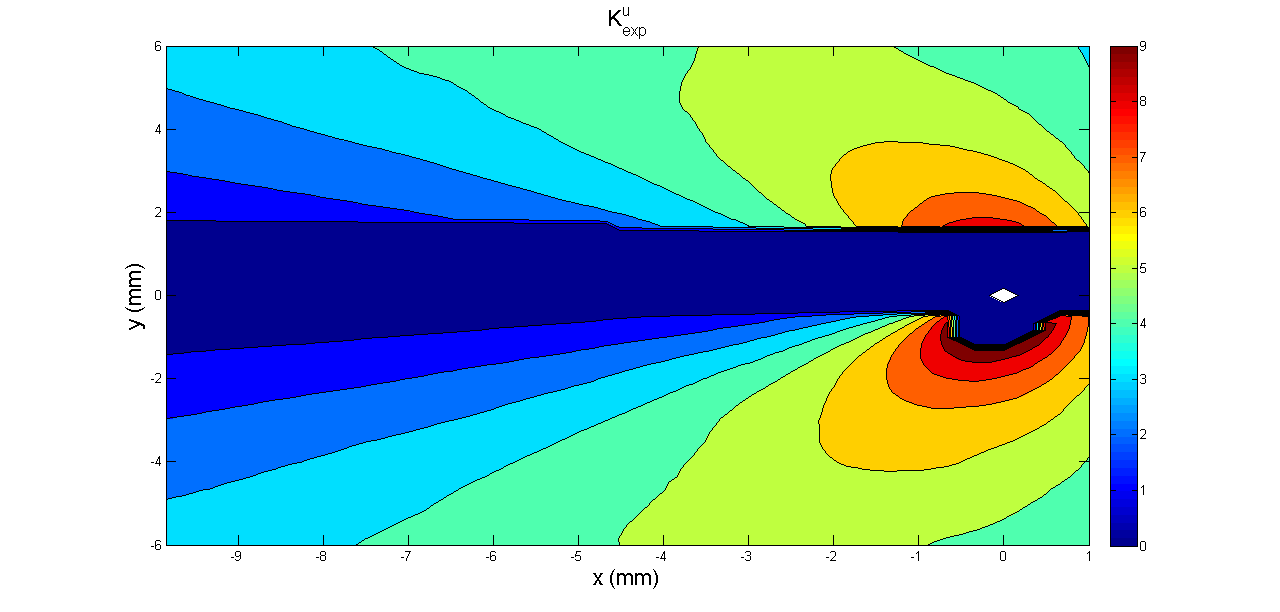
\includegraphics[width=1\textwidth]{K_U_T.png}
	\caption{Contour plot of experimental values $K_1^U$.  Values above above 10 have been set to 0 for clarity}
	\label{fig:kU}
\end{figure}

\begin{figure}[H]
	\centering
	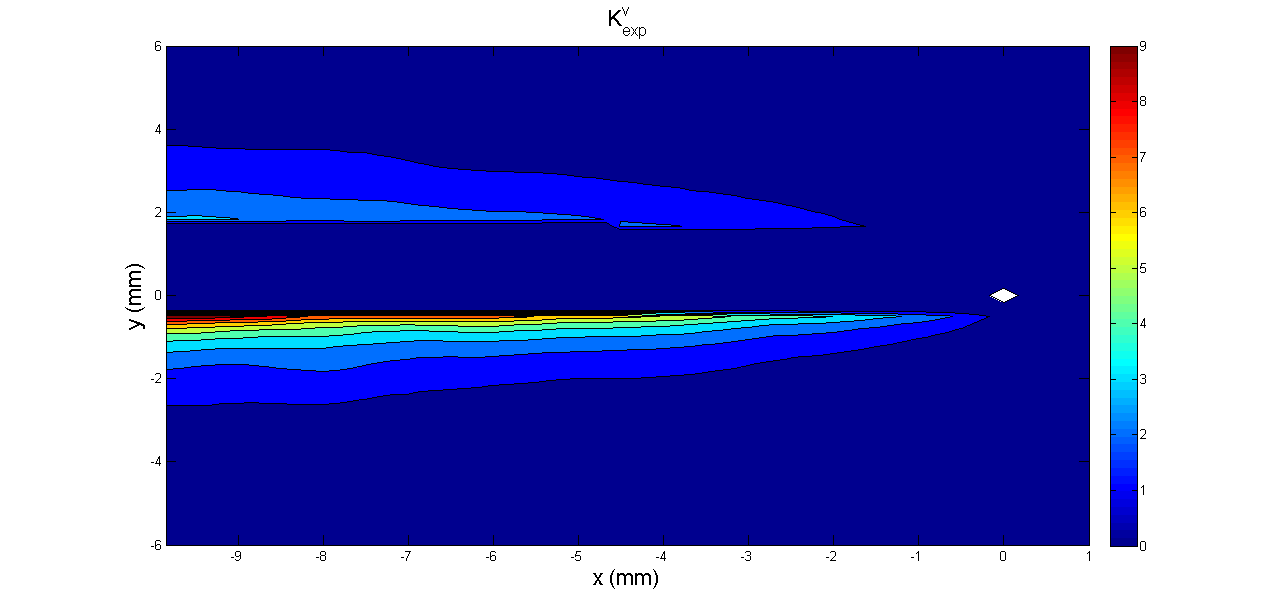
\includegraphics[width=1\textwidth]{K_V_T.png}
	\caption{Contour plot of experimental values $K_1^V$. Values above above 10 have been set to 0 for clarity}
	\label{fig:kV}
\end{figure}

Experimental $K_I$ values were observed to be highly dependent on location. $K_I$ became less accurate as distance from the crack increased for values calculated from $u_x$ data. The opposite relation was observed for $u_y$ data. To analyze how well theoretical $K_I$ fit the experimental data, two points along the x-axis on the $K_I^{u_x}$ plot were chosen for further analysis. $K_I$ was then calculated for each of the eight load increments. Results are shown in Figure \ref{fig:K1}. $K_I$ at both locations closely matched predicted values with $R^2>0.98$ in both cases. 



\begin{figure}[H]
	\begin{center}
		
		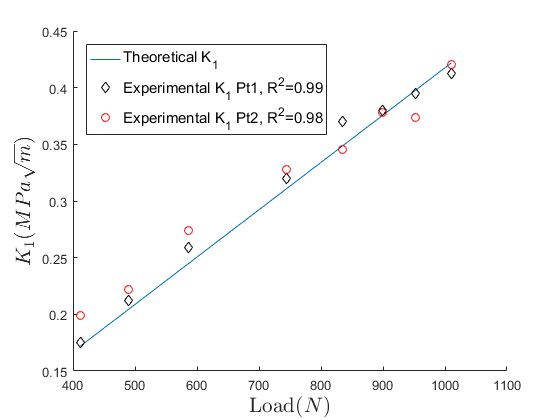
\includegraphics[width=1\textwidth]{K_1_Comparisons.png}
		\caption{Theoretical and experimental mode I stress intensity factor at two points along the x-axis.}
		\label{fig:K1}
	\end{center}
\end{figure}

Contour plots of raw $u_x$ and $u_y$ displacement data were drawn and shown in Figure \ref{cc1} and Figure \ref{fig:cc2}. 

\begin{figure}[H]
	\centering
	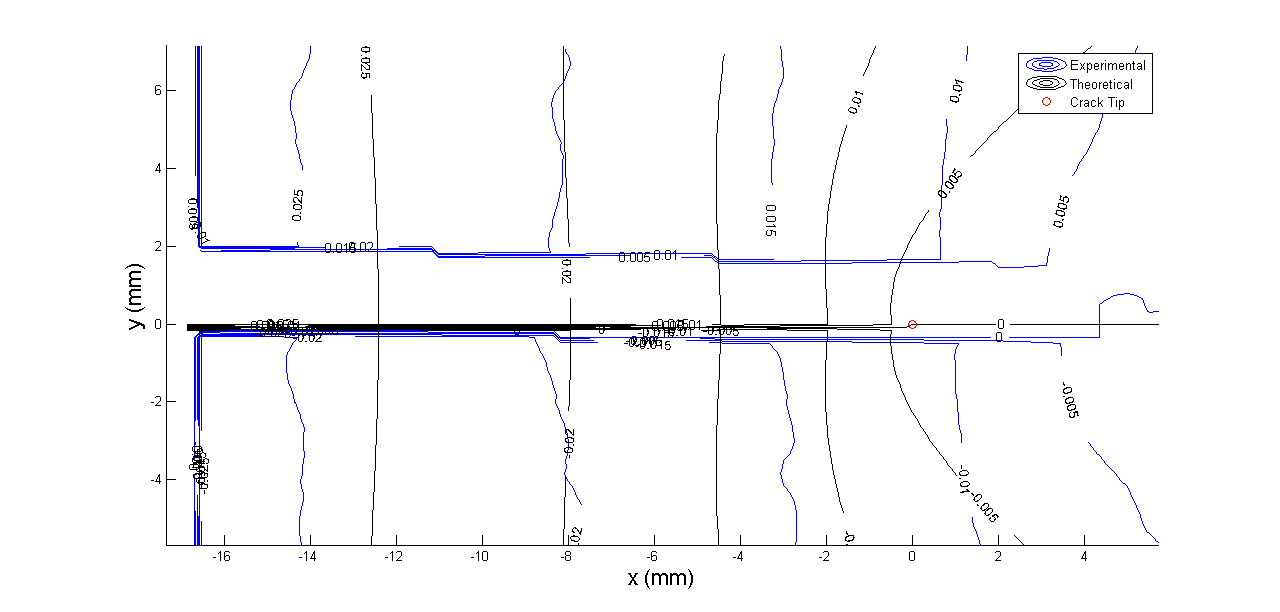
\includegraphics[width=1\textwidth]{contourCompare_8_1.png}
	\caption{Comparison between theoretical and experimental U displacements}
	\label{fig:cc1}
\end{figure}

\begin{figure}[H]
	\centering
	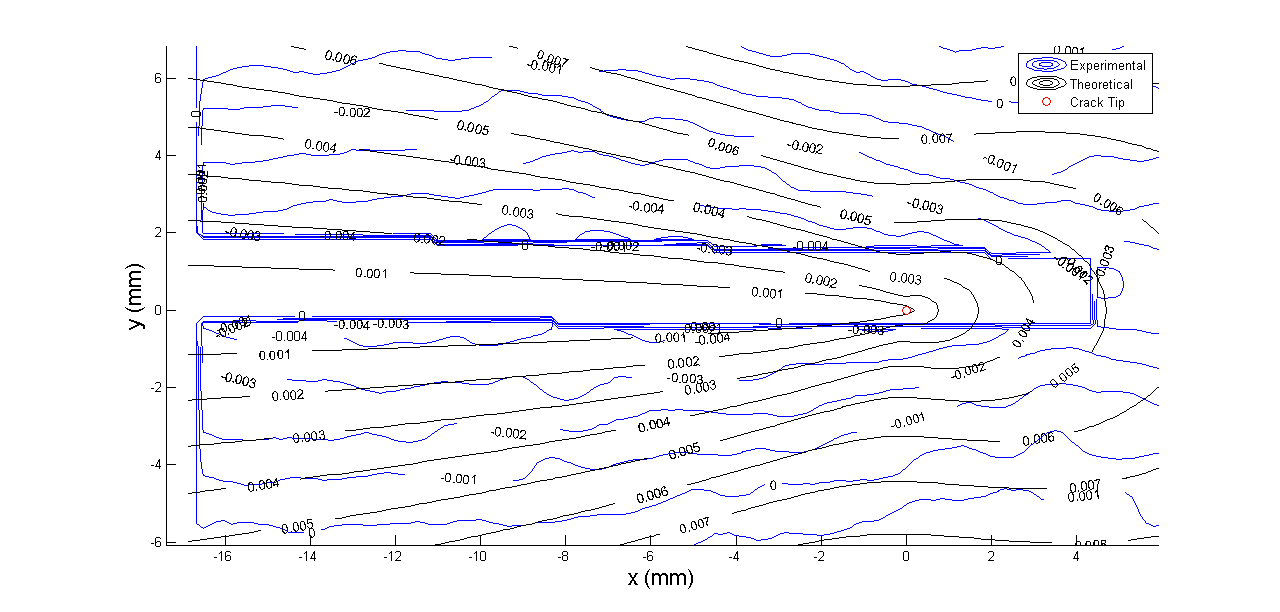
\includegraphics[width=1\textwidth]{contourCompare_8_2.png}
	\caption{Comparison between theoretical and experimental V displacements}
	\label{fig:cc2}
\end{figure}


\section{Discussion}%Nik
The general shape of both $u_x$ and $u_y$ fields in Mode I tests matched well with predictions. Field magnitudes also agreed closely, but spacing between contour lines did not always match perfectly. The roughness in experimental contours is likely due to errors inherent in DIC methods such as finite pixel/speckle size and subset selection. There are several possible explanations for disagreements in contour spacing. First, theoretical calculations depend on bulk modulus, $\mu$, which was not measured, but derived from Young's Modulus and Poisson's ratio, taken from on-line sources. Additionally, theoretical calculations assume an infinitely thin crack with a sharp tip. The test specimen crack was cut with a band saw and therefore has a finite width and a blunted tip. 
\section{Conclusion}%Nick

\section{Figures}
% DIC setup
\begin{figure}[H]
	\centering
	\includegraphics[width=1\textwidth]{DIC_Setup.png}
	\caption{The specimen is mounted to the fixture with the DIC system in place, here the camera is fixed to a tripod and two adjustable lights are seen on either side.}
	\label{fig:DIC}
\end{figure}

% Mode I Specimen geometry
\begin{figure}[H]
	\centering
	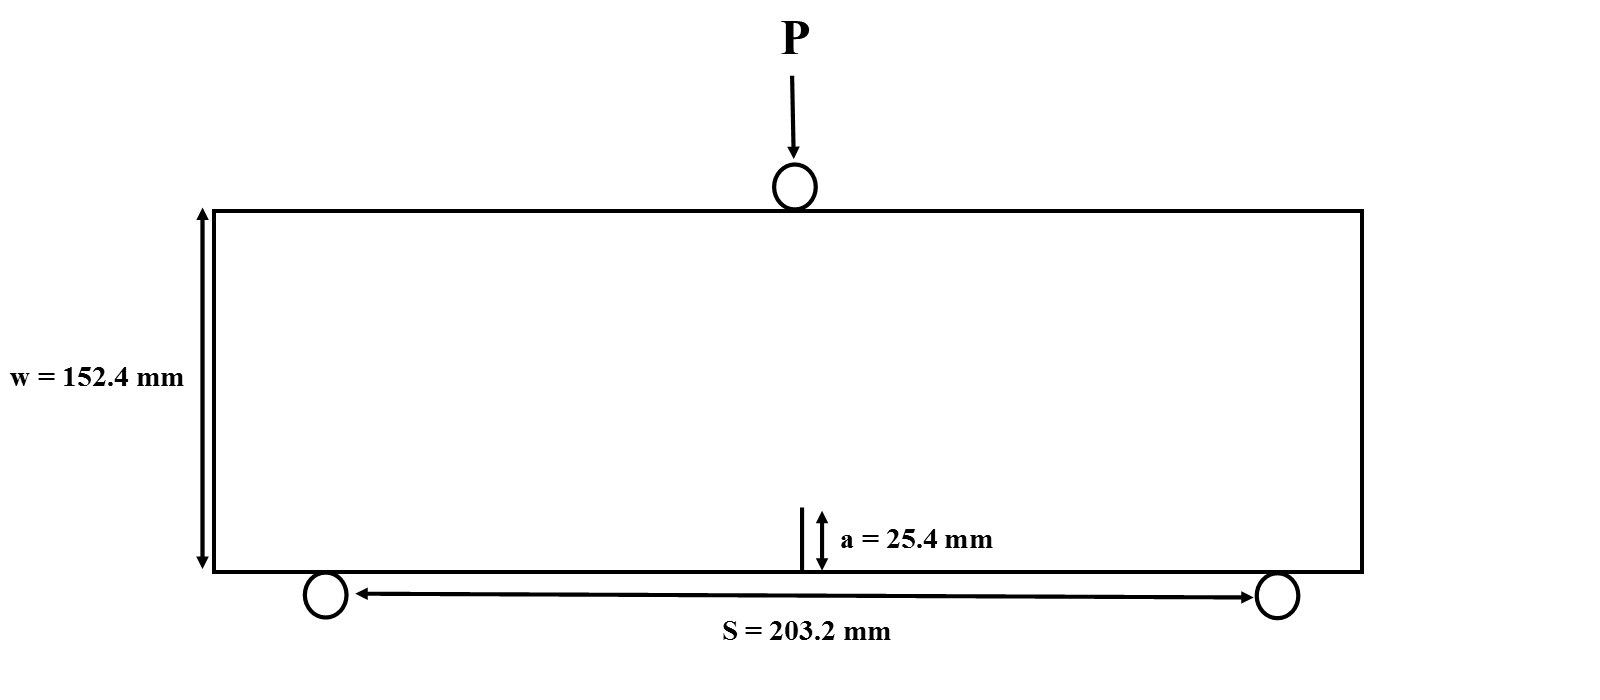
\includegraphics[width=1\textwidth]{Geometry.png}
	\caption{Three point loading configuration of specimen, where S = 0.2032 m, w = 0.1524 m, a = 0.0254 m and a specimen thickness (B) of 0.00875 m. Applied load, P, is applied to the top roller}
	\label{fig:Geometry}
\end{figure}

% Mixed Mode Specimen Geometry
\begin{figure}[H]
	\centering
	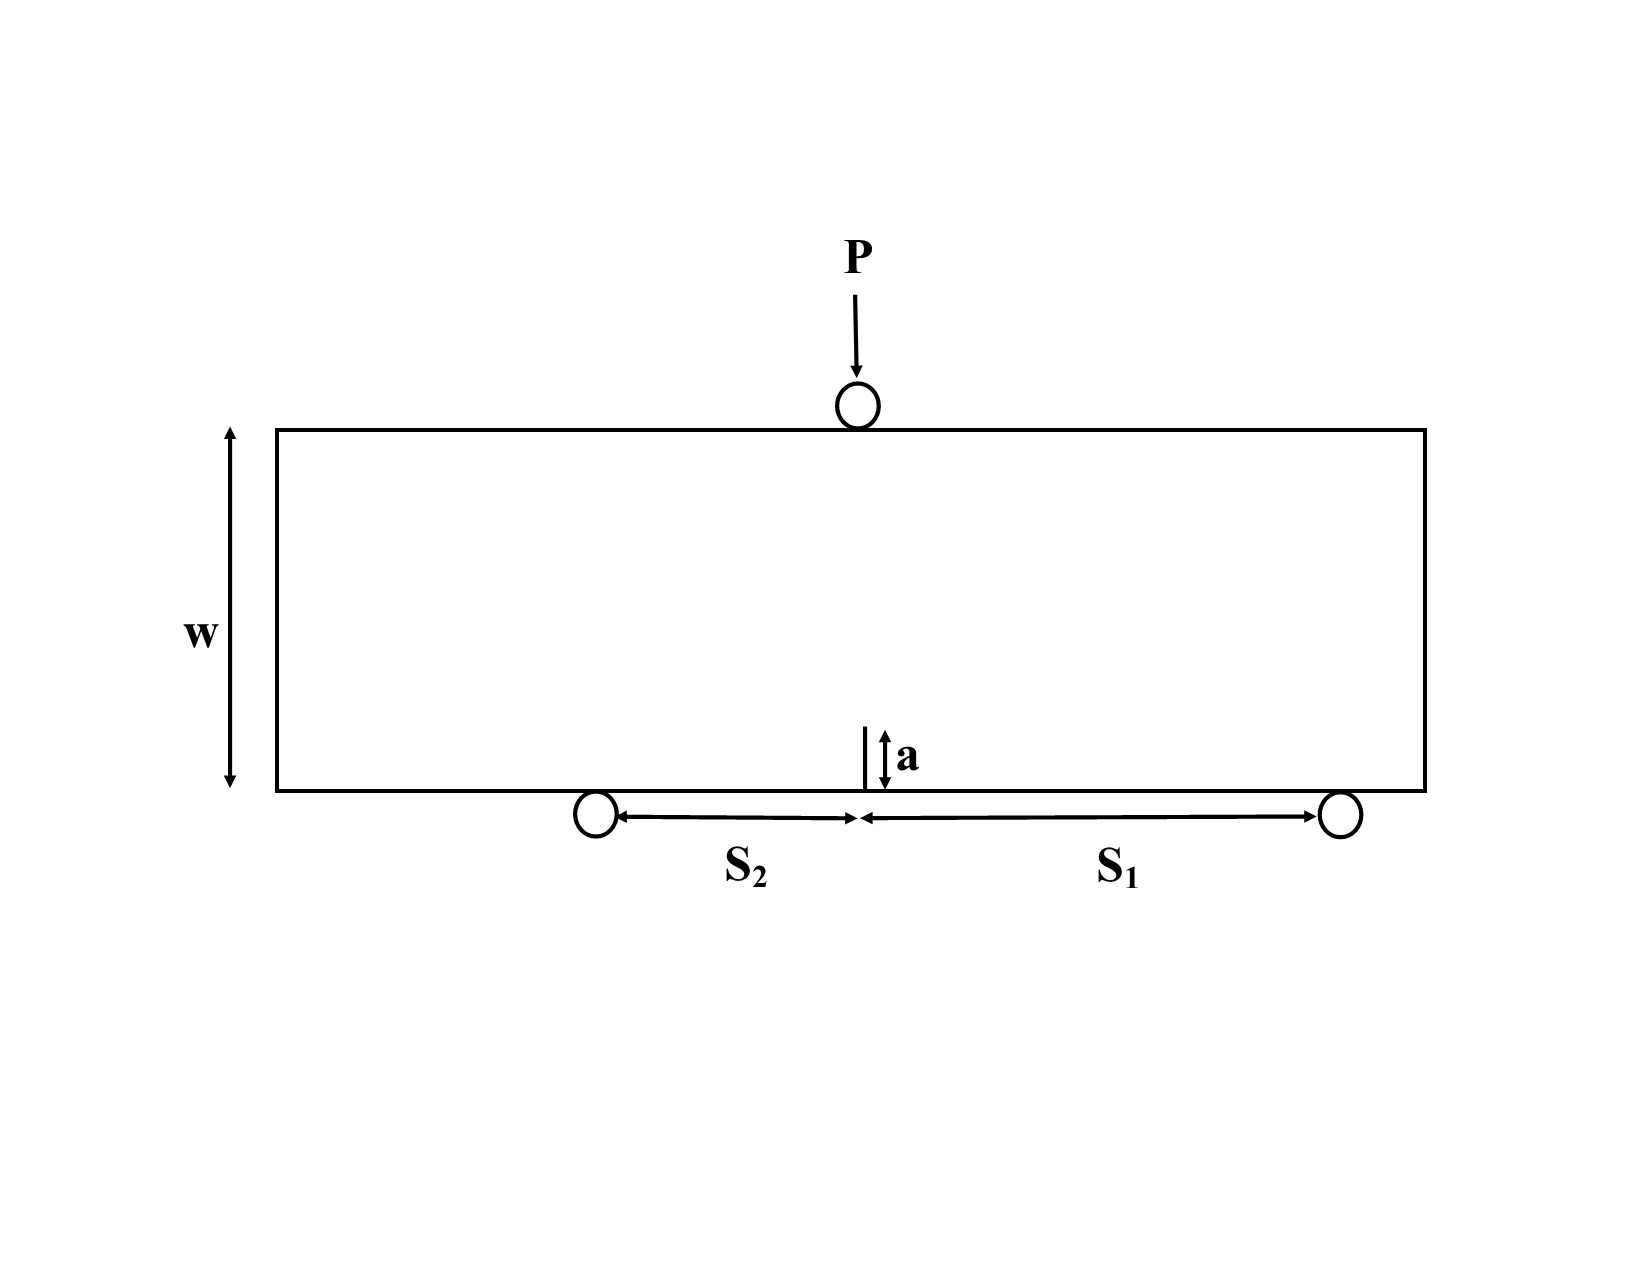
\includegraphics[width=1\textwidth]{Geometry_Mixed.png}
	\caption{Three point loading configuration of specimen, where $S_{1}$ = 0.1016 m, $S_{2}$ = 0.0508 m, w = 0.1524 m, a = 0.0254 m, and a specimen thickness (B) of 0.00875 m. Applied load, P, is applied to the top roller}
	\label{fig:Geometry_Mixed}
\end{figure}
% DIC setup
\begin{figure}[H]
	\centering
	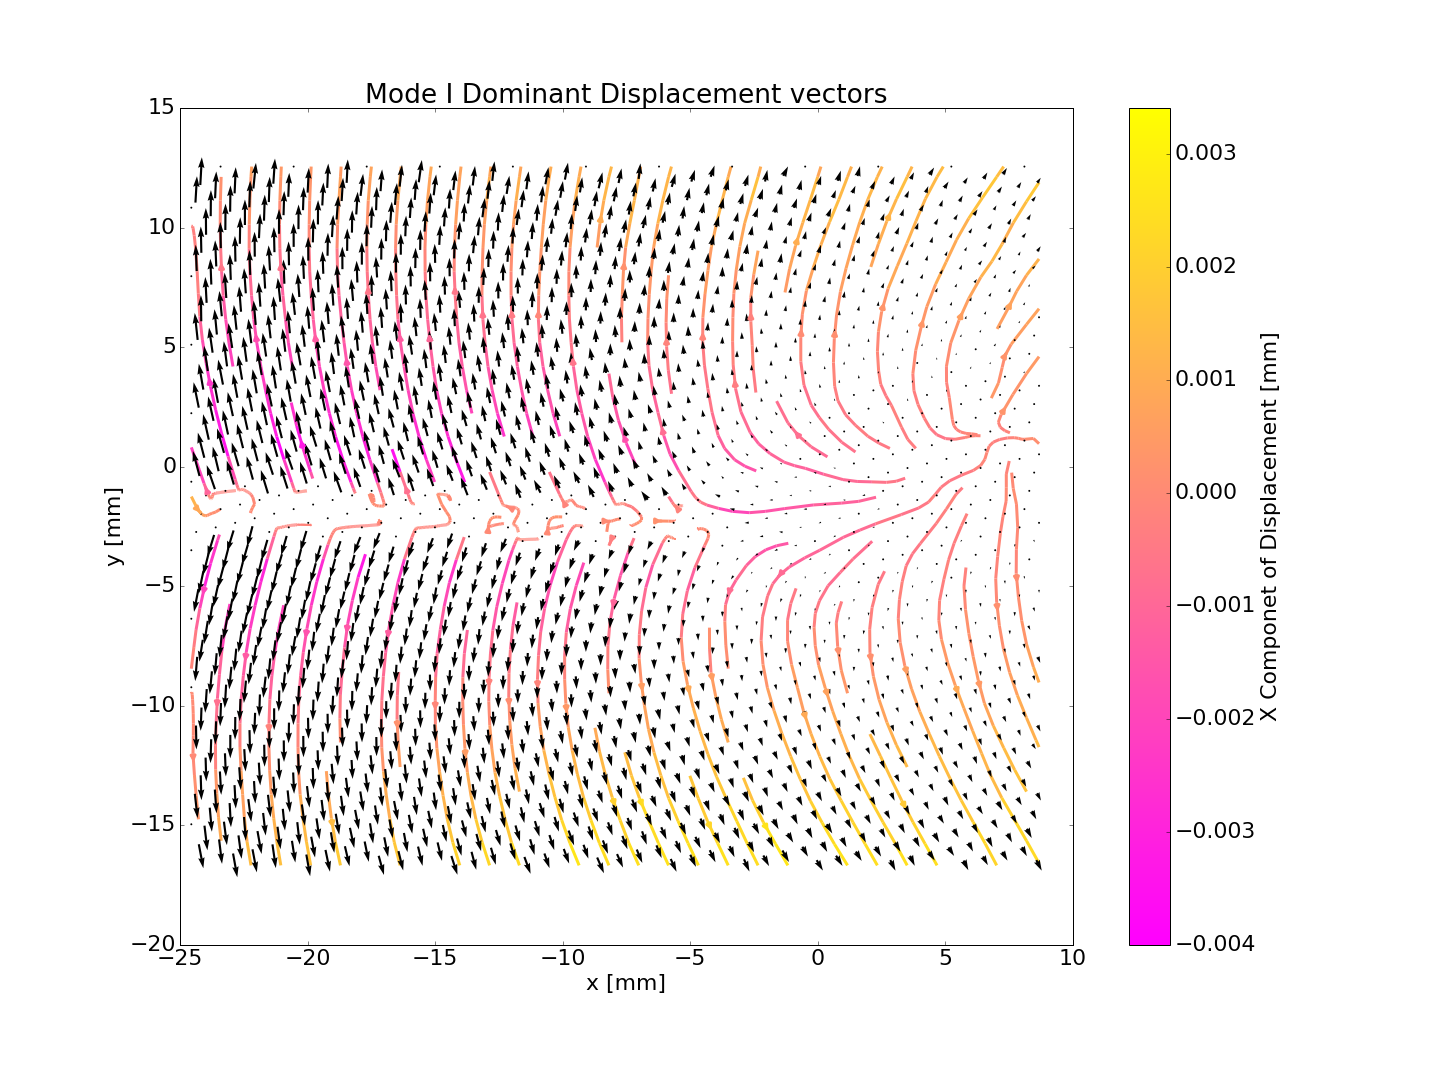
\includegraphics[width=1\textwidth]{quiverMixedMode.png}
	\caption{Displacements vectors around crack for an asymmetric load 587 N.}
	\label{fig:QuiverMix}
\end{figure}
% DIC setup
\begin{figure}[H]
	\centering
	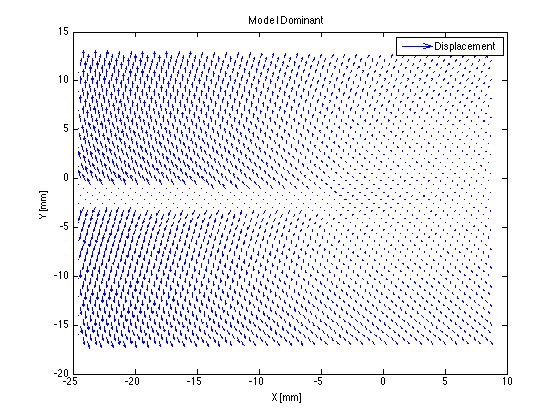
\includegraphics[width=1\textwidth]{QuiverModeI.png}
	\caption{Displacements vectors around crack tip for a symmetric load of 534.7 N }
	\label{fig:Quiver1}
\end{figure}

	 
\section{Tables}
Recoded Experimental Data:
\begin{table}[h]\footnotesize
	\centering
	\begin{tabular}{ |l|l|l|l| }
		\hline
		\multicolumn{2}{|c|}{\textbf{Mode I}}&\multicolumn{2}{|c|}{\textbf{Mixed Mode}}\\ \hline
		\textbf{Load [N]} & \textbf{Image Number}&\textbf{Load [N]} & \textbf{Image Number}\\  \hline
		0-5 & 7.784 & 0-4 & 25.58 \\ \hline
		6& 7.784 & 5 & 27.58 \\ \hline
		7 & 93.77 & 6 & 86 \\ \hline
		8 & 215.6 & 7 &191.7 \\ \hline
		9 & 295 & 8 & 324 \\ \hline
		10 & 412 & 9 & 431 \\ \hline
		11 & 489.6 & 10 & 486 \\ \hline
		12 & 587 & 11 & 534.7 \\ \hline
		13 & 745 & 12 & 629.1 \\ \hline
		14 & 834 & 13 & 761.7 \\ \hline
		15 & 899 & 14 & 805.3 \\ \hline
		16 & 952 & 15 & 849.6 \\ \hline
		17 & 1010 & 16 & 896 \\ \hline
		-	& - & 17 & 1000 \\ \hline
		
		
		
	\end{tabular}
	\caption{Loads and associated image number, first few images were used as reference images.}
	\label{tab:data}
\end{table}
% All layups
\
\section{Appendix}

\subsection{Code}

\begin{verbatim}

\end{verbatim}


\bibliographystyle{IEEEtran}
\bibliography{Lab2Bib}
\end{document}